%%%%%%%%%%%%%%%%%%%%%%%%%%%%%%%%%%%%%%%%%%%%%%%%%%%%%%%%%%%%%%%%%%%%%%%%%%%%%%%%%%
\begin{frame}[fragile]\frametitle{}
\begin{center}
{\Large TensorFlow for Machine Learning}
\end{center}
\end{frame}

%%%%%%%%%%%%%%%%%%%%%%%%%%%%%%%%%%%%%%%%%%%%%%%%%%%%%%%%%%%%%%%%%%%%%%%%
\begin{frame}[fragile]\frametitle{TensorFlow Paradigm}
\begin{itemize}
\item Although popular for Deep Learning, TensorFlow is actually a very generic graph computation library.
\item For Machine Learning, TensorFlow Estimators provided.
\end{itemize}

\begin{center}
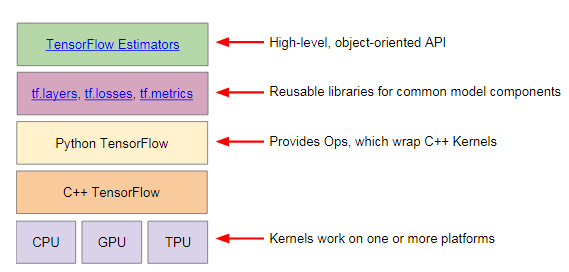
\includegraphics[width=0.8\linewidth,keepaspectratio]{tfest}
\end{center}

\end{frame}

%%%%%%%%%%%%%%%%%%%%%%%%%%%%%%%%%%%%%%%%%%%%%%%%%%%%%%%%%%
\begin{frame}[fragile]\frametitle{Example}
\begin{lstlisting}
import tensorflow as tf

# Set up a linear classifier.
classifier = tf.estimator.LinearClassifier()

# Train the model on some example data.
classifier.train(input_fn=train_input_fn, steps=2000)

# Use it to predict.
predictions = classifier.predict(input_fn=predict_input_fn)
\end{lstlisting}
\end{frame}


%%%%%%%%%%%%%%%%%%%%%%%%%%%%%%%%%%%%%%%%%%%%%%%%%%%%%%%%%%
\begin{frame}[fragile]\frametitle{California Housing Data Set Example}
Load the necessary libraries:
\begin{lstlisting}
import math

from IPython import display
from matplotlib import cm
from matplotlib import gridspec
from matplotlib import pyplot as plt
import numpy as np
import pandas as pd
from sklearn import metrics
import tensorflow as tf
from tensorflow.python.data import Dataset

tf.logging.set_verbosity(tf.logging.ERROR)
pd.options.display.max_rows = 10
pd.options.display.float_format = '{:.1f}'.format
\end{lstlisting}

(Ref: https://colab.research.google.com/notebooks/mlcc/first\_steps\_with\_tensor\_flow.ipynb?)
\end{frame}


%%%%%%%%%%%%%%%%%%%%%%%%%%%%%%%%%%%%%%%%%%%%%%%%%%%%%%%%%%
\begin{frame}[fragile]\frametitle{Load the dataset}
\begin{lstlisting}
california_housing_dataframe = pd.read_csv("https://storage.googleapis.com/ml_universities/california_housing_train.csv", sep=",")
\end{lstlisting}
\end{frame}

%%%%%%%%%%%%%%%%%%%%%%%%%%%%%%%%%%%%%%%%%%%%%%%%%%%%%%%%%%
\begin{frame}[fragile]\frametitle{California Housing Data Set Example}
Randomize the dataset and scale median\_house\_value to be in units of thousands, so it can be learned a little more easily with learning rates in a range that we usually use.
\begin{lstlisting}
california_housing_dataframe = california_housing_dataframe.reindex(
    np.random.permutation(california_housing_dataframe.index))
california_housing_dataframe["median_house_value"] /= 1000.0
print(california_housing_dataframe.head())
\end{lstlisting}
17000 rows x 9 columns
\end{frame}

%%%%%%%%%%%%%%%%%%%%%%%%%%%%%%%%%%%%%%%%%%%%%%%%%%%%%%%%%%
\begin{frame}[fragile]\frametitle{Examine the dataset}

\begin{lstlisting}
print(california_housing_dataframe.describe())
\end{lstlisting}
17000 rows x 9 columns
\end{frame}

%%%%%%%%%%%%%%%%%%%%%%%%%%%%%%%%%%%%%%%%%%%%%%%%%%%%%%%%%%
\begin{frame}[fragile]\frametitle{California Housing Data Set Example}
We'll try to predict median\_house\_value, which will be our label (sometimes also called a target). We'll use total\_rooms as our input feature.
\begin{lstlisting}
# Define the input feature: total_rooms.
my_feature = california_housing_dataframe[["total_rooms"]]

# Configure a numeric feature column for total_rooms.
feature_columns = [tf.feature_column.numeric_column("total_rooms")]

# Define the label.
targets = california_housing_dataframe["median_house_value"]
\end{lstlisting}

\end{frame}

%%%%%%%%%%%%%%%%%%%%%%%%%%%%%%%%%%%%%%%%%%%%%%%%%%%%%%%%%%
\begin{frame}[fragile]\frametitle{Configure the LinearRegressor}
\begin{lstlisting}
# Use gradient descent as the optimizer for training the model.
my_optimizer=tf.train.GradientDescentOptimizer(learning_rate=0.0000001)
my_optimizer = tf.contrib.estimator.clip_gradients_by_norm(my_optimizer, 5.0)

# Configure the linear regression model with our feature columns and optimizer.
# Set a learning rate of 0.0000001 for Gradient Descent.
linear_regressor = tf.estimator.LinearRegressor(
    feature_columns=feature_columns,
    optimizer=my_optimizer
)
\end{lstlisting}

\end{frame}

%%%%%%%%%%%%%%%%%%%%%%%%%%%%%%%%%%%%%%%%%%%%%%%%%%%%%%%%%%
\begin{frame}[fragile]\frametitle{Define the Input Function}
\begin{itemize}
\item  We are training this model using the GradientDescentOptimizer, which implements Mini-Batch Stochastic Gradient Descent (SGD). 
\item The learning\_rate argument controls the size of the gradient step.
\item To be safe, we also apply gradient clipping to our optimizer via clip\_gradients\_by\_norm. 
\item Gradient clipping ensures the magnitude of the gradients do not become too large during training, which can cause gradient descent to fail.
\end{itemize}
\end{frame}

%%%%%%%%%%%%%%%%%%%%%%%%%%%%%%%%%%%%%%%%%%%%%%%%%%%%%%%%%%
\begin{frame}[fragile]\frametitle{Optimizer}
\begin{itemize}
\item  We are training this model using the GradientDescentOptimizer, which implements Mini-Batch Stochastic Gradient Descent (SGD). 
\item The learning\_rate argument controls the size of the gradient step.
\item To be safe, we also apply gradient clipping to our optimizer via clip\_gradients\_by\_norm. 
\item Gradient clipping ensures the magnitude of the gradients do not become too large during training, which can cause gradient descent to fail.
\end{itemize}
\end{frame}


%%%%%%%%%%%%%%%%%%%%%%%%%%%%%%%%%%%%%%%%%%%%%%%%%%%%%%%%%%
\begin{frame}[fragile]\frametitle{Define the Input Function}
\begin{itemize}
\item  To import our California housing data into our LinearRegressor, we need to define an input function, 
\item Which instructs TensorFlow how to preprocess the data, as well as how to batch, shuffle, and repeat it during model training.
\item First, we'll convert our pandas feature data into a dict of NumPy arrays. 
\item We can then use the TensorFlow Dataset API to construct a dataset object from our data
\item Then break our data into batches of batch\_size, to be repeated for the specified number of epochs (num\_epochs).
\end{itemize}
\end{frame}

%%%%%%%%%%%%%%%%%%%%%%%%%%%%%%%%%%%%%%%%%%%%%%%%%%%%%%%%%%
\begin{frame}[fragile]\frametitle{Define the Input Function}
NOTE:
\begin{itemize}
\item  When the default value of \lstinline|num_epochs=None| is passed to \lstinline|repeat()|, the input data will be repeated indefinitely.

\item Next, if $shuffle$ is set to True, we'll shuffle the data so that it's passed to the model randomly during training. The \lstinline|buffer_size| argument specifies the size of the dataset from which shuffle will randomly sample.

\item Finally, our input function constructs an iterator for the dataset and returns the next batch of data to the LinearRegressor.
\end{itemize}
\end{frame}


%%%%%%%%%%%%%%%%%%%%%%%%%%%%%%%%%%%%%%%%%%%%%%%%%%%%%%%%%%
\begin{frame}[fragile]\frametitle{Define the Input Function}
\begin{lstlisting}
def my_input_fn(features, targets, batch_size=1, shuffle=True, num_epochs=None):
    # Convert pandas data into a dict of np arrays.
    features = {key:np.array(value) for key,value in dict(features).items()}                                           
 
    # Construct a dataset, and configure batching/repeating
    ds = Dataset.from_tensor_slices((features,targets)) # warning: 2GB limit
    ds = ds.batch(batch_size).repeat(num_epochs)
    
    # Shuffle the data, if specified
    if shuffle:
      ds = ds.shuffle(buffer_size=10000)
    
    # Return the next batch of data
    features, labels = ds.make_one_shot_iterator().get_next()
    return features, labels
\end{lstlisting}

\end{frame}


%%%%%%%%%%%%%%%%%%%%%%%%%%%%%%%%%%%%%%%%%%%%%%%%%%%%%%%%%%
\begin{frame}[fragile]\frametitle{Train the Model}
\begin{itemize}
\item We can now call train() on our linear\_regressor to train the model. 
\item We'll wrap my\_input\_fn in a lambda so we can pass in my\_feature and target as arguments, 
\item and to start, we'll train for 100 steps.
\end{itemize}

\begin{lstlisting}
_ = linear_regressor.train(
    input_fn = lambda:my_input_fn(my_feature, targets),
    steps=100
)
\end{lstlisting}

\end{frame}

%%%%%%%%%%%%%%%%%%%%%%%%%%%%%%%%%%%%%%%%%%%%%%%%%%%%%%%%%%
\begin{frame}[fragile]\frametitle{Evaluate the Model}
\begin{itemize}
\item Let's make predictions on that training data, to see how well our model fit it during training.
\item Training error measures how well your model fits the training data, but it does not measure how well your model generalizes to new data. 
\item Later, need to see how to split your data to evaluate your model's ability to generalize.
\end{itemize}
\end{frame}

%%%%%%%%%%%%%%%%%%%%%%%%%%%%%%%%%%%%%%%%%%%%%%%%%%%%%%%%%%
\begin{frame}[fragile]\frametitle{Evaluate the Model}
 Create an input function for predictions.
\begin{lstlisting}
prediction_input_fn =lambda: my_input_fn(my_feature, targets, num_epochs=1, shuffle=False)

# Call predict() on the linear_regressor to make predictions.
predictions = linear_regressor.predict(input_fn=prediction_input_fn)

# Format predictions as a NumPy array, so we can calculate error metrics.
predictions = np.array([item['predictions'][0] for item in predictions])

mean_squared_error = metrics.mean_squared_error(predictions, targets)
root_mean_squared_error = math.sqrt(mean_squared_error)
print "Mean Squared Error (on training data): %0.3f" % mean_squared_error
print "Root Mean Squared Error (on training data): %0.3f" % root_mean_squared_error
\end{lstlisting}

\end{frame}

%%%%%%%%%%%%%%%%%%%%%%%%%%%%%%%%%%%%%%%%%%%%%%%%%%%%%%%%%%
\begin{frame}[fragile]\frametitle{Evaluate the Model}
\begin{itemize}
\item Is this a good model? How would you judge how large this error is?
\item Mean Squared Error (MSE) can be hard to interpret, so we often look at Root Mean Squared Error (RMSE) instead. 
\item A nice property of RMSE is that it can be interpreted on the same scale as the original targets.
\end{itemize}
\end{frame}

%%%%%%%%%%%%%%%%%%%%%%%%%%%%%%%%%%%%%%%%%%%%%%%%%%%%%%%%%%
\begin{frame}[fragile]\frametitle{Evaluate the Model}
Let's compare the RMSE to the difference of the min and max of our targets:
\begin{lstlisting}
min_house_value = california_housing_dataframe["median_house_value"].min()
max_house_value = california_housing_dataframe["median_house_value"].max()
min_max_difference = max_house_value - min_house_value

\end{lstlisting}
Min. Median House Value: 14.999
Max. Median House Value: 500.001
Difference between Min. and Max.: 485.002
Root Mean Squared Error: 237.417

Our error spans nearly half the range of the target values. Can we do better?
\end{frame}

%%%%%%%%%%%%%%%%%%%%%%%%%%%%%%%%%%%%%%%%%%%%%%%%%%%%%%%%%%
\begin{frame}[fragile]\frametitle{Evaluate the Model}
Let's compare the RMSE to the difference of the min and max of our targets:
\begin{lstlisting}
min_house_value = california_housing_dataframe["median_house_value"].min()
max_house_value = california_housing_dataframe["median_house_value"].max()
min_max_difference = max_house_value - min_house_value

print "Min. Median House Value: %0.3f" % min_house_value
print "Max. Median House Value: %0.3f" % max_house_value
print "Difference between Min. and Max.: %0.3f" % min_max_difference
print "Root Mean Squared Error: %0.3f" % root_mean_squared_error
\end{lstlisting}
Min. Median House Value: 14.999
Max. Median House Value: 500.001
Difference between Min. and Max.: 485.002
Root Mean Squared Error: 237.417

Our error spans nearly half the range of the target values. Can we do better?
\end{frame}

%%%%%%%%%%%%%%%%%%%%%%%%%%%%%%%%%%%%%%%%%%%%%%%%%%%%%%%%%%
\begin{frame}[fragile]\frametitle{Evaluate the Model}
Let's see how well our predictions match our targets, in terms of overall summary statistics.
\begin{lstlisting}
calibration_data = pd.DataFrame()
calibration_data["predictions"] = pd.Series(predictions)
calibration_data["targets"] = pd.Series(targets)
print(calibration_data.describe())
\end{lstlisting}

\begin{center}
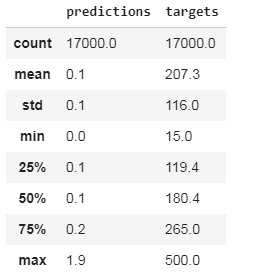
\includegraphics[width=0.4\linewidth,keepaspectratio]{rmse1}
\end{center}
Way off.
\end{frame}

%%%%%%%%%%%%%%%%%%%%%%%%%%%%%%%%%%%%%%%%%%%%%%%%%%%%%%%%%%
\begin{frame}[fragile]\frametitle{Evaluate the Model}
\begin{itemize}
\item We can also visualize the data and the line we've learned. 
\item Recall that linear regression on a single feature can be drawn as a line mapping input x to output y.
\item First, we'll get a uniform random sample of the data so we can make a readable scatter plot.
\end{itemize}

\begin{lstlisting}
sample = california_housing_dataframe.sample(n=300)
\end{lstlisting}
\end{frame}


%%%%%%%%%%%%%%%%%%%%%%%%%%%%%%%%%%%%%%%%%%%%%%%%%%%%%%%%%%
\begin{frame}[fragile]\frametitle{Visualize the Data}
We'll plot the line we've learned, drawing from the model's bias term and feature weight, together with the scatter plot. The line will show up red.
\begin{lstlisting}
# Get the min and max total_rooms values.
x_0 = sample["total_rooms"].min()
x_1 = sample["total_rooms"].max()

# Retrieve the final weight and bias generated during training.
weight = linear_regressor.get_variable_value('linear/linear_model/total_rooms/weights')[0]
bias = linear_regressor.get_variable_value('linear/linear_model/bias_weights')

# Get the predicted median_house_values for the min and max total_rooms values.
y_0 = weight * x_0 + bias 
y_1 = weight * x_1 + bias

# Plot our regression line from (x_0, y_0) to (x_1, y_1).
plt.plot([x_0, x_1], [y_0, y_1], c='r')

# Label the graph axes.
plt.ylabel("median_house_value")
plt.xlabel("total_rooms")

# Plot a scatter plot from our data sample.
plt.scatter(sample["total_rooms"], sample["median_house_value"])

# Display graph.
plt.show()
\end{lstlisting}
\end{frame}

%%%%%%%%%%%%%%%%%%%%%%%%%%%%%%%%%%%%%%%%%%%%%%%%%%%%%%%%%%
\begin{frame}[fragile]\frametitle{Evaluate the Model}
\begin{center}
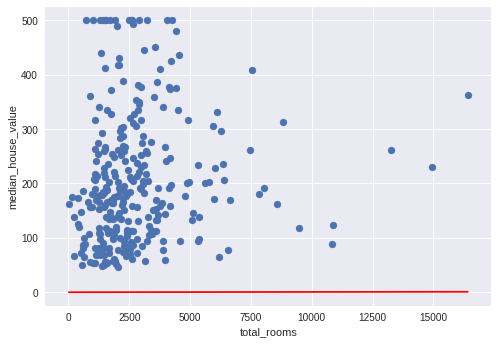
\includegraphics[width=0.8\linewidth,keepaspectratio]{rmse2}
\end{center}
This initial line looks way off. 
\end{frame}

%%%%%%%%%%%%%%%%%%%%%%%%%%%%%%%%%%%%%%%%%%%%%%%%%%%%%%%%%%
\begin{frame}[fragile]\frametitle{Tweak the Model Hyperparameters}
\begin{itemize}
\item In this function, we'll proceed in 10 evenly divided periods so that we can observe the model improvement at each period.
\item 
For each period, we'll compute and graph training loss. This may help you judge when a model is converged, or if it needs more iterations.
\item 
We'll also plot the feature weight and bias term values learned by the model over time. This is another way to see how things converge.
\end{itemize}

\end{frame}

%%%%%%%%%%%%%%%%%%%%%%%%%%%%%%%%%%%%%%%%%%%%%%%%%%%%%%%%%%
\begin{frame}[fragile]\frametitle{Tweak the Model Hyperparameters}
\begin{lstlisting}
def train_model(learning_rate, steps, batch_size, input_feature="total_rooms"):
  periods = 10
  steps_per_period = steps / periods

  my_feature = input_feature
  my_feature_data = california_housing_dataframe[[my_feature]]
  my_label = "median_house_value"
  targets = california_housing_dataframe[my_label]
\end{lstlisting}
\end{frame}

%%%%%%%%%%%%%%%%%%%%%%%%%%%%%%%%%%%%%%%%%%%%%%%%%%%%%%%%%%
\begin{frame}[fragile]\frametitle{Tweak the Model Hyperparameters}
\begin{lstlisting}
  # Create feature columns
  feature_columns = [tf.feature_column.numeric_column(my_feature)]
  
  # Create input functions
  training_input_fn = lambda:my_input_fn(my_feature_data, targets, batch_size=batch_size)
  prediction_input_fn = lambda: my_input_fn(my_feature_data, targets, num_epochs=1, shuffle=False)
  
  # Create a linear regressor object.
  my_optimizer = tf.train.GradientDescentOptimizer(learning_rate=learning_rate)
  my_optimizer = tf.contrib.estimator.clip_gradients_by_norm(my_optimizer, 5.0)
  linear_regressor = tf.estimator.LinearRegressor(
      feature_columns=feature_columns,
      optimizer=my_optimizer
  )

\end{lstlisting}
\end{frame}

%%%%%%%%%%%%%%%%%%%%%%%%%%%%%%%%%%%%%%%%%%%%%%%%%%%%%%%%%%
\begin{frame}[fragile]\frametitle{Tweak the Model Hyperparameters}
\begin{lstlisting}

  # Set up to plot the state of our model's line each period.
  plt.figure(figsize=(15, 6))
  plt.subplot(1, 2, 1)
  plt.title("Learned Line by Period")
  plt.ylabel(my_label)
  plt.xlabel(my_feature)
  sample = california_housing_dataframe.sample(n=300)
  plt.scatter(sample[my_feature], sample[my_label])
  colors = [cm.coolwarm(x) for x in np.linspace(-1, 1, periods)]
\end{lstlisting}
\end{frame}


%%%%%%%%%%%%%%%%%%%%%%%%%%%%%%%%%%%%%%%%%%%%%%%%%%%%%%%%%%
\begin{frame}[fragile]\frametitle{Tweak the Model Hyperparameters}
\begin{lstlisting}
# Train the model, but do so inside a loop so that we can periodically assess
  # loss metrics.
  print "Training model..."
  print "RMSE (on training data):"
  root_mean_squared_errors = []
  for period in range (0, periods):
    # Train the model, starting from the prior state.
    linear_regressor.train(
        input_fn=training_input_fn,
        steps=steps_per_period
    )
    # Take a break and compute predictions.
    predictions = linear_regressor.predict(input_fn=prediction_input_fn)
    predictions = np.array([item['predictions'][0] for item in predictions])
\end{lstlisting}
\end{frame}

%%%%%%%%%%%%%%%%%%%%%%%%%%%%%%%%%%%%%%%%%%%%%%%%%%%%%%%%%%
\begin{frame}[fragile]\frametitle{Tweak the Model Hyperparameters}
\begin{lstlisting}
# Compute loss.
    root_mean_squared_error = math.sqrt(
        metrics.mean_squared_error(predictions, targets))
    # Occasionally print the current loss.
    print "  period %02d : %0.2f" % (period, root_mean_squared_error)
    # Add the loss metrics from this period to our list.
    root_mean_squared_errors.append(root_mean_squared_error)
    # Finally, track the weights and biases over time.
    # Apply some math to ensure that the data and line are plotted neatly.
    y_extents = np.array([0, sample[my_label].max()])
\end{lstlisting}
\end{frame}

%%%%%%%%%%%%%%%%%%%%%%%%%%%%%%%%%%%%%%%%%%%%%%%%%%%%%%%%%%
\begin{frame}[fragile]\frametitle{Tweak the Model Hyperparameters}
\begin{lstlisting}
   weight = linear_regressor.get_variable_value('linear/linear_model/%s/weights' % input_feature)[0]
    bias = linear_regressor.get_variable_value('linear/linear_model/bias_weights')

    x_extents = (y_extents - bias) / weight
    x_extents = np.maximum(np.minimum(x_extents,
                                      sample[my_feature].max()),
                           sample[my_feature].min())
    y_extents = weight * x_extents + bias
    plt.plot(x_extents, y_extents, color=colors[period]) 
  print "Model training finished."
\end{lstlisting}
\end{frame}

%%%%%%%%%%%%%%%%%%%%%%%%%%%%%%%%%%%%%%%%%%%%%%%%%%%%%%%%%%
\begin{frame}[fragile]\frametitle{Tweak the Model Hyperparameters}
\begin{lstlisting}
# Output a graph of loss metrics over periods.
  plt.subplot(1, 2, 2)
  plt.ylabel('RMSE')
  plt.xlabel('Periods')
  plt.title("Root Mean Squared Error vs. Periods")
  plt.tight_layout()
  plt.plot(root_mean_squared_errors)

  # Output a table with calibration data.
  calibration_data = pd.DataFrame()
  calibration_data["predictions"] = pd.Series(predictions)
  calibration_data["targets"] = pd.Series(targets)
  display.display(calibration_data.describe())

  print "Final RMSE (on training data): %0.2f" % root_mean_squared_error
\end{lstlisting}
\end{frame}

%%%%%%%%%%%%%%%%%%%%%%%%%%%%%%%%%%%%%%%%%%%%%%%%%%%%%%%%%%
\begin{frame}[fragile]\frametitle{Task 1: Achieve an RMSE of 180 or Below}
\begin{lstlisting}
train_model(
    learning_rate=0.00001,
    steps=100,
    batch_size=1
)

Training model...
RMSE (on training data):
  period 00 : 236.32
  period 01 : 235.11
  period 02 : 233.90
  period 03 : 232.70
  period 04 : 231.50
  period 05 : 230.31
  period 06 : 229.13
  period 07 : 227.96
  period 08 : 226.79
  period 09 : 225.63
Model training finished.
\end{lstlisting}

\end{frame}



%%%%%%%%%%%%%%%%%%%%%%%%%%%%%%%%%%%%%%%%%%%%%%%%%%%%%%%%%%
\begin{frame}[fragile]\frametitle{Evaluate the Model}
\begin{center}
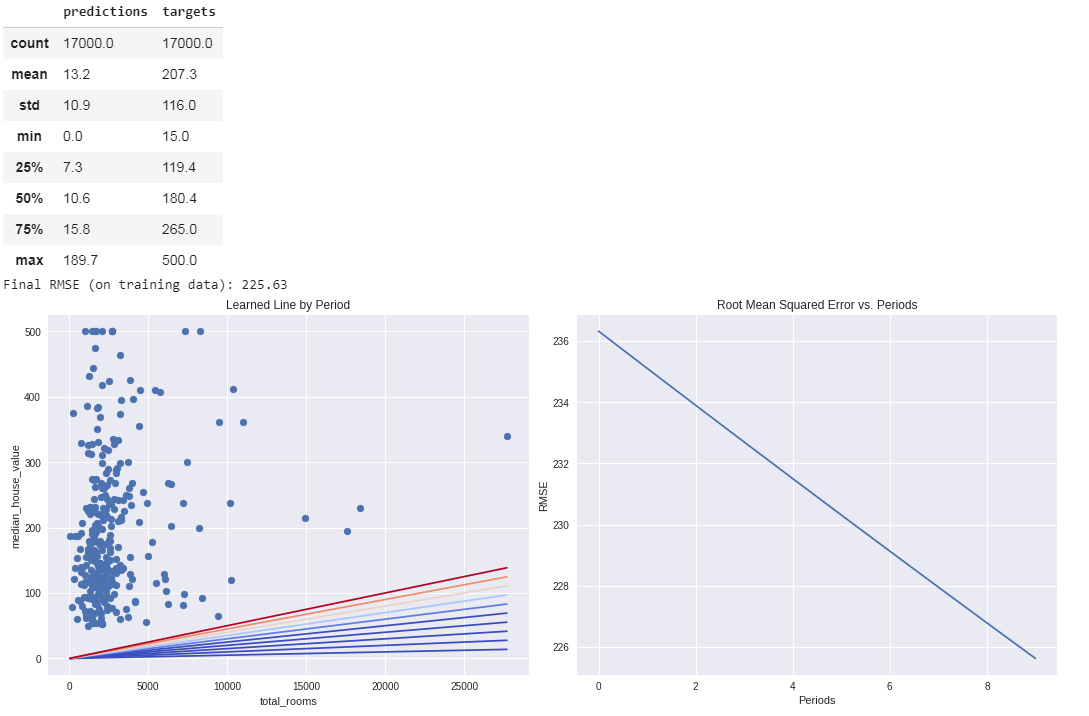
\includegraphics[width=\linewidth,keepaspectratio]{rmse3}
\end{center}
Still off. 
\end{frame}

%%%%%%%%%%%%%%%%%%%%%%%%%%%%%%%%%%%%%%%%%%%%%%%%%%%%%%%%%%
\begin{frame}[fragile]\frametitle{See if this works?}
\begin{lstlisting}
train_model(
    learning_rate=0.00002,
    steps=500,
    batch_size=5
)

Training model...
RMSE (on training data):
  period 00 : 225.63
  period 01 : 214.42
  period 02 : 204.04
  period 03 : 194.62
  period 04 : 187.23
  period 05 : 180.53
  period 06 : 175.88
  period 07 : 171.74
  period 08 : 169.08
  period 09 : 167.45
Model training finished.
\end{lstlisting}
It does. There may be other combinations of settings that also give good results.
\end{frame}

%%%%%%%%%%%%%%%%%%%%%%%%%%%%%%%%%%%%%%%%%%%%%%%%%%%%%%%%%%
\begin{frame}[fragile]\frametitle{Evaluate the Model}
\begin{center}
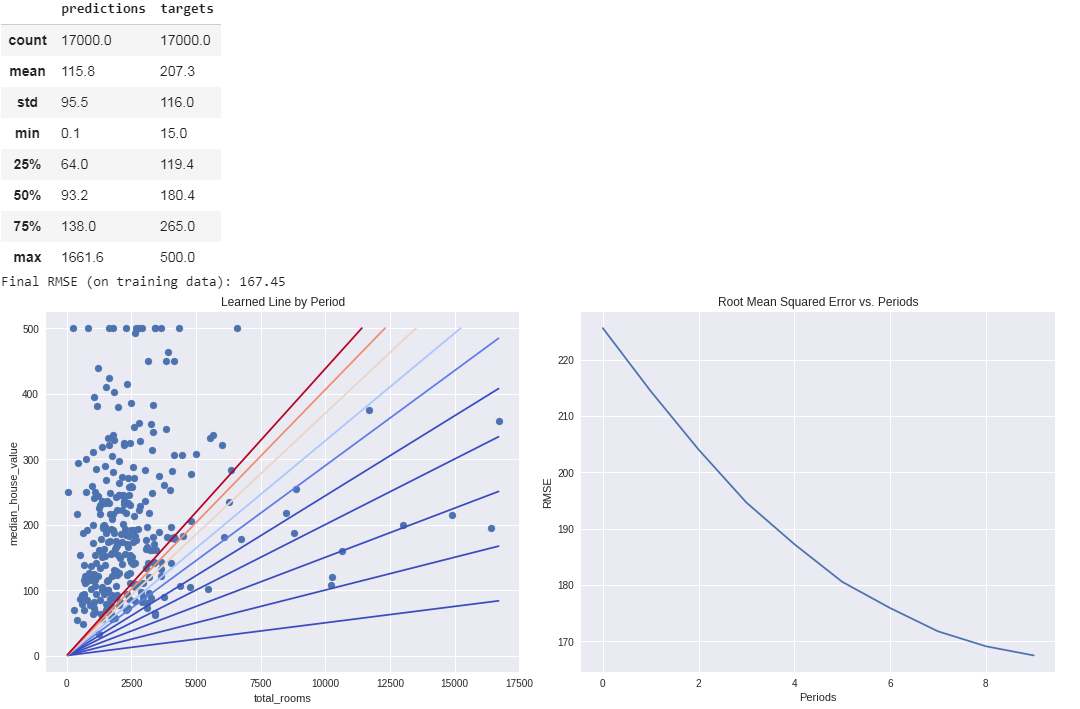
\includegraphics[width=\linewidth,keepaspectratio]{rmse4}
\end{center}
Acceptable.
\end{frame}


%%
%%
%%
%%
%%
%%
%%%%%%%%%%%%%%%%%%%%%%%%%%%%%%%%%%%%%%%%%%%%%%%%%%%%%%%%%%%%%%%%%%%%%%%%%%
%%\begin{frame}[fragile]\frametitle{Scikit-Learn's Estimator API}
%%The steps in using the Scikit-Learn estimator API are as follows
%%\begin{itemize}
%%\item Choose a class of model by importing the appropriate estimator class from Scikit-Learn.
%%\item Choose model hyper-parameters by instantiating this class.
%%\item Arrange data into a features matrix and target vector.
%%\item Fit the model to your data by calling the fit() method of the model instance.
%%\begin{itemize}
%%    \item For supervised learning, predict labels for unknown data using the predict().
%%    \item For unsupervised learning, transform or infer properties of the data using transform() or predict().
%%\end{itemize}
%%\end{itemize}
%%\end{frame}
%%
%%%%%%%%%%%%%%%%%%%%%%%%%%%%%%%%%%%%%%%%%%%%%%%%%%%%%%%%%%%%%%%%%%%%%%%%%%
%%\begin{frame}[fragile]\frametitle{}
%%\begin{itemize}
%%\item The \texttt{Estimator.fit} method sets the state of the estimator based on the training data. 
%%\item Usually, the data is comprised of a two-dimensional numpy array X of shape \texttt{(n\_samples, n\_predictors) }that holds the so-called feature matrix and a one-dimensional numpy array y that holds the responses. 
%%\item Some estimators allow the user to control the fitting behavior. 
%%\end{itemize}
%%\end{frame}
%%
%%%%%%%%%%%%%%%%%%%%%%%%%%%%%%%%%%%%%%%%%%%%%%%%%%%%%%%%%%%%
%%\begin{frame}[fragile]\frametitle{Estimator}
%%\begin{lstlisting}
%%class Estimator(object):
%%    def fit(self, X, y=None):
%%        """Fits estimator to data. """
%%        # set state of ''self''
%%        return self
%%    def predict(self, X):
%%        """Predict response of ''X''. """
%%        # compute predictions ''pred''
%%        return pred
%%\end{lstlisting}
%%\begin{itemize}
%%\item fit(X,y) sets the state of the estimator.
%%\item  X is usually a 2D numpy array of shape (num\_samples, num\_features).
%%\item  y is a 1D array with shape (n\_samples,)
%%\item  predict(X) returns the class or value
%%%\item  predict\_proba() returns a 2D array of shape (n\_samples, n\_classes)
%%\end{itemize}
%%\end{frame}
%%
%%%%%%%%%%%%%%%%%%%%%%%%%%%%%%%%%%%%%%%%%%%%%%%%%%%%%%%%%%%%
%%\begin{frame}[fragile]\frametitle{Regression: Linear regression}
%%\begin{lstlisting}
%%from sklearn.linear_model import LinearRegression
%%import matplotlib.pyplot as plt
%%
%%model = LinearRegression(normalize=True)
%%
%%x = np.arange(10)
%%y = 2 * x + 1
%%plt.plot(x, y, 'o');
%%plt.show()
%%
%%# The input data for sklearn is 2D: 
%%# (samples == 3 x features == 1)
%%X = x[:, np.newaxis]
%%
%%model.fit(X, y)
%%
%%x1 = np.array([1,23,10,14])
%%X1 = x1[:, np.newaxis]
%%y_pred = model.predict(X1)
%%
%%print(model.coef_)
%%print(model.intercept_)
%%print(model.residues_)
%%\end{lstlisting}
%%\end{frame}
%%
%%
%%
%%
%%%
%%%%%%%%%%%%%%%%%%%%%%%%%%%%%%%%%%%%%%%%%%%%%%%%%%%%%%%%%%%%%
%%%\begin{frame}[fragile]\frametitle{Model}
%%%\begin{lstlisting}
%%%from sklearn import svm
%%%
%%%estimator = svm.SVC(gamma=0.001)
%%%
%%%estimator.fit(X, y)
%%%
%%%y_pred = estimator.predict(x)
%%%
%%%\end{lstlisting}
%%%\end{frame}
%%
%%
%%%%%%%%%%%%%%%%%%%%%%%%%%%%%%%%%%%%%%%%%%%%%%%%%%%%%%%%%%%%
%%\begin{frame}[fragile]\frametitle{Cross Validation}
%%\begin{lstlisting}
%%from sklearn import metrics
%%from sklearn import cross_validation as cv
%%
%%X_train, X_test, y_train, y_test     
%%	= cv.train_test_split(X, y, test_size=0.2)
%%
%%model      = ClassifierEstimator()
%%
%%model.fit(X_train, y_train)
%%
%%expected   = y_test
%%
%%predicted  = model.predict(X_test)
%%
%%print(metrics.classification_report(expected, predicted))
%%print(metrics.confusion_matrix(expected, predicted))
%%print(metrics.f1_score(expected, predicted))
%%\end{lstlisting}
%%\end{frame}
%%
%%
%%%%%%%%%%%%%%%%%%%%%%%%%%%%%%%%%%%%%%%%%%%%%%%%%%%%%%%%%%%%
%%\begin{frame}[fragile]\frametitle{Coefficient of Determination}
%%\begin{lstlisting}
%%from sklearn import metrics
%%from sklearn import cross_validation as cv
%%
%%splits     = cv.train_test_split(X, y, test_size=0.2)
%%X_train, X_test, y_train, y_test = splits
%%
%%model      = RegressionEstimator()
%%
%%model.fit(X_train, y_train)
%%
%%expected   = y_test
%%
%%predicted  = model.predict(y_test)
%%
%%print(metrics.mean_squared_error(expected, predicted))
%%print(metrics.r2_score(expected, predicted))
%%\end{lstlisting}
%%\end{frame}
%%
%%%%%%%%%%%%%%%%%%%%%%%%%%%%%%%%%%%%%%%%%%%%%%%%%%%%%%%%%%%%%
%%%\begin{frame}[fragile]\frametitle{Classification Example}
%%%K nearest neighbors (kNN) is a supervised clustering/classification algorithm. Which group the unseen point belongs to, is classified.
%%%\begin{lstlisting}
%%%from sklearn import neighbors, datasets
%%%
%%%iris = datasets.load_iris()
%%%X, y = iris.data, iris.target
%%%
%%%knn = neighbors.KNeighborsClassifier(n_neighbors=5)
%%%
%%%knn.fit(X, y)
%%%
%%%result = knn.predict([[3, 5, 4, 2],])
%%%
%%%print(iris.target_names[result])
%%%
%%%knn.predict_proba([[3, 5, 4, 2],])
%%%\end{lstlisting}
%%%\end{frame}
%%%%%%%%%%%%%%%%%%%%%%%%%%%%%%%%%%%%%%%%%%%%%%%%%%%%%%%%%%%%
%%\begin{frame}[fragile]\frametitle{Classifier: Support Vector Machine}
%%
%%\begin{lstlisting}
%%from sklearn.svm import SVC
%%
%%model = SVC(kernel=``rbf'', C=1.0, gamma=1e-4)
%%
%%model.fit(X_train, y_train)
%%
%%predicted = model.predict(X_test)
%%
%%expected   = y_test
%%
%%from sklearn.metrics import f1_score
%%
%%print(f1_score(expected, predicted))
%%\end{lstlisting}
%%\end{frame}
%%
%%
%%
%%%%%%%%%%%%%%%%%%%%%%%%%%%%%%%%%%%%%%%%%%%%%%%%%%%%%%%%%%%%
%%\begin{frame}[fragile]\frametitle{Classifier: K-Nearest neighbor classifier}
%%For any unknown quantity, returns the label of the closest training point.
%%
%%\begin{lstlisting}
%%from sklearn.neighbors import KNeighborsClassifier
%%
%%X, y = iris.data, iris.target
%%
%%clf = KNeighborsClassifier(n_neighbors=1)
%%
%%clf.fit(X, y)
%%
%%y_pred = clf.predict(X)
%%
%%print(np.all(y == y_pred))
%%
%%from sklearn.metrics import confusion_matrix
%%
%%print(confusion_matrix(y, y_pred))
%%\end{lstlisting}
%%\end{frame}
%%
%%
%%
%%%%%%%%%%%%%%%%%%%%%%%%%%%%%%%%%%%%%%%%%%%%%%%%%%%%%%%%%%%%
%%\begin{frame}[fragile]\frametitle{Dimensionality Reduction: PCA}
%%Principle Component Analysis (PCA) is a dimension reduction technique.
%%\begin{lstlisting}
%%X, y = iris.data, iris.target
%%from sklearn.decomposition import PCA
%%pca = PCA(n_components=2)
%%pca.fit(X)
%%X_reduced = pca.transform(X)
%%print("Reduced dataset shape:", X_reduced.shape)
%%
%%\end{lstlisting}
%%%
%%%import pylab as pl
%%%pl.scatter(X_reduced[:, 0], X_reduced[:, 1], c=y, cmap='RdYlBu')
%%%
%%%print("Meaning of the 2 components:")
%%%for component in pca.components_:
%%%    	print(" + ".join("%.3f x %s" % (value, name) for value, name in zip(component, iris.feature_names)))
%%%    	
%%\end{frame}
%%
%%%%%%%%%%%%%%%%%%%%%%%%%%%%%%%%%%%%%%%%%%%%%%%%%%%%%%%%%%%%
%%\begin{frame}[fragile]\frametitle{Clustering: K-means}
%%Clustering groups together observations that are homogeneous with respect to a given criterion.
%%\begin{lstlisting}
%%from sklearn.cluster import KMeans
%%
%%k_means = KMeans(n_clusters=3, random_state=0) 
%%
%%k_means.fit(X)
%%
%%y_pred = k_means.predict(X)
%%
%%pl.scatter(X_reduced[:, 0], X_reduced[:, 1], c=y_pred,
%%           cmap='RdYlBu');
%%\end{lstlisting}
%%\end{frame}
%%
%%
%%
%%
%%%%%%%%%%%%%%%%%%%%%%%%%%%%%%%%%%%%%%%%%%%%%%%%%%%%%%%%%%%%
%%\begin{frame}[fragile]\frametitle{Quick Application: Optical Character Recognition}
%%Loading and visualizing the digits data:
%%\begin{lstlisting}
%%from sklearn import datasets
%%import matplotlib.pyplot as plt
%%
%%digits = datasets.load_digits()
%%print(digits.images.shape)
%%
%%fig, axes = plt.subplots(10, 10, figsize=(8, 8))
%%fig.subplots_adjust(hspace=0.1, wspace=0.1)
%%
%%for i, ax in enumerate(axes.flat):
%%    ax.imshow(digits.images[i], cmap='binary')
%%    ax.text(0.05, 0.05, str(digits.target[i]),
%%            transform=ax.transAxes, color='green')
%%    ax.set_xticks([])
%%    ax.set_yticks([])
%%
%%plt.show()
%%\end{lstlisting}
%%\end{frame}
%%
%%
%%%%%%%%%%%%%%%%%%%%%%%%%%%%%%%%%%%%%%%%%%%%%%%%%%%%%%%%%%%%
%%\begin{frame}[fragile]\frametitle{The images themselves}
%%Here the data is simply each pixel value within an 8x8 grid:
%%\begin{lstlisting}
%%print(digits.images.shape)
%%print(digits.images[0])
%%
%%(1797, 8, 8)
%%[[  0.   0.   5.  13.   9.   1.   0.   0.]
%% [  0.   0.  13.  15.  10.  15.   5.   0.]
%% [  0.   3.  15.   2.   0.  11.   8.   0.]
%% [  0.   4.  12.   0.   0.   8.   8.   0.]
%% [  0.   5.   8.   0.   0.   9.   8.   0.]
%% [  0.   4.  11.   0.   1.  12.   7.   0.]
%% [  0.   2.  14.   5.  10.  12.   0.   0.]
%% [  0.   0.   6.  13.  10.   0.   0.   0.]]
%%
%%\end{lstlisting}
%%So our data have 1797 samples in 64 dimensions.
%%\end{frame}
%%%
%%%%%%%%%%%%%%%%%%%%%%%%%%%%%%%%%%%%%%%%%%%%%%%%%%%%%%%%%%%%%
%%%\begin{frame}[fragile]\frametitle{Unsupervised Learning: Dimensionality Reduction}
%%%We'd like to visualize our points within the 64-dimensional parameter space, but it's difficult to plot points in 64 dimensions! Instead we'll reduce the dimensions to 2, using an unsupervised method. Here, we'll make use of a manifold learning algorithm called Isomap, and transform the data to two dimensions.
%%%\begin{lstlisting}
%%%from sklearn.manifold import Isomap
%%%
%%%iso = Isomap(n_components=2)
%%%
%%%data_projected = iso.fit_transform(digits.data)
%%%
%%%print(data_projected.shape)
%%%
%%%plt.scatter(data_projected[:, 0], data_projected[:, 1], c=digits.target,
%%%            edgecolor='none', alpha=0.5, cmap=plt.cm.get_cmap('nipy_spectral', 10));
%%%plt.colorbar(label='digit label', ticks=range(10))
%%%plt.clim(-0.5, 9.5)
%%%\end{lstlisting}
%%%
%%%\end{frame}
%%
%%
%%%%%%%%%%%%%%%%%%%%%%%%%%%%%%%%%%%%%%%%%%%%%%%%%%%%%%%%%%%%
%%\begin{frame}[fragile]\frametitle{Classification on Digits}
%%The first thing we'll want to do is split the digits into a training and testing sample:
%%\begin{lstlisting}
%%from sklearn.cross_validation import train_test_split
%%
%%Xtrain, Xtest, ytrain, ytest = train_test_split(digits.data, digits.target,random_state=2)
%%
%%print(Xtrain.shape, Xtest.shape)
%%
%%from sklearn.linear_model import LogisticRegression
%%
%%clf = LogisticRegression(penalty='l2')
%%
%%clf.fit(Xtrain, ytrain)
%%
%%ypred = clf.predict(Xtest)
%%
%%from sklearn.metrics import accuracy_score
%%accuracy_score(ytest, ypred)
%%
%%\end{lstlisting}
%%
%%\end{frame}
%%
%%%%%%%%%%%%%%%%%%%%%%%%%%%%%%%%%%%%%%%%%%%%%%%%%%%%%%%%%%%%%
%%%\begin{frame}[fragile]\frametitle{Results}
%%%\begin{lstlisting}
%%%plt.imshow(np.log(confusion_matrix(ytest, ypred)),
%%%           cmap='Blues', interpolation='nearest')
%%%plt.grid(False)
%%%plt.ylabel('true')
%%%plt.xlabel('predicted');
%%%\end{lstlisting}
%%%\begin{center}
%%%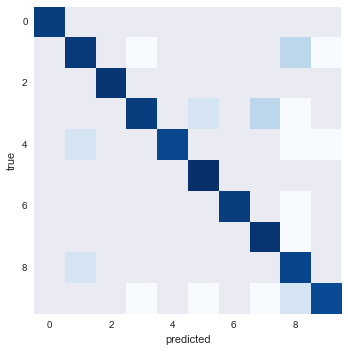
\includegraphics[width=0.5\linewidth,keepaspectratio]{optresult}
%%%\end{center}
%%%\end{frame}
%%
